% Options for packages loaded elsewhere
\PassOptionsToPackage{unicode}{hyperref}
\PassOptionsToPackage{hyphens}{url}
\PassOptionsToPackage{dvipsnames,svgnames,x11names}{xcolor}
%
\documentclass[
  letterpaper,
  DIV=11,
  numbers=noendperiod]{scrartcl}

\usepackage{amsmath,amssymb}
\usepackage{iftex}
\ifPDFTeX
  \usepackage[T1]{fontenc}
  \usepackage[utf8]{inputenc}
  \usepackage{textcomp} % provide euro and other symbols
\else % if luatex or xetex
  \usepackage{unicode-math}
  \defaultfontfeatures{Scale=MatchLowercase}
  \defaultfontfeatures[\rmfamily]{Ligatures=TeX,Scale=1}
\fi
\usepackage{lmodern}
\ifPDFTeX\else  
    % xetex/luatex font selection
\fi
% Use upquote if available, for straight quotes in verbatim environments
\IfFileExists{upquote.sty}{\usepackage{upquote}}{}
\IfFileExists{microtype.sty}{% use microtype if available
  \usepackage[]{microtype}
  \UseMicrotypeSet[protrusion]{basicmath} % disable protrusion for tt fonts
}{}
\makeatletter
\@ifundefined{KOMAClassName}{% if non-KOMA class
  \IfFileExists{parskip.sty}{%
    \usepackage{parskip}
  }{% else
    \setlength{\parindent}{0pt}
    \setlength{\parskip}{6pt plus 2pt minus 1pt}}
}{% if KOMA class
  \KOMAoptions{parskip=half}}
\makeatother
\usepackage{xcolor}
\setlength{\emergencystretch}{3em} % prevent overfull lines
\setcounter{secnumdepth}{5}
% Make \paragraph and \subparagraph free-standing
\ifx\paragraph\undefined\else
  \let\oldparagraph\paragraph
  \renewcommand{\paragraph}[1]{\oldparagraph{#1}\mbox{}}
\fi
\ifx\subparagraph\undefined\else
  \let\oldsubparagraph\subparagraph
  \renewcommand{\subparagraph}[1]{\oldsubparagraph{#1}\mbox{}}
\fi

\usepackage{color}
\usepackage{fancyvrb}
\newcommand{\VerbBar}{|}
\newcommand{\VERB}{\Verb[commandchars=\\\{\}]}
\DefineVerbatimEnvironment{Highlighting}{Verbatim}{commandchars=\\\{\}}
% Add ',fontsize=\small' for more characters per line
\usepackage{framed}
\definecolor{shadecolor}{RGB}{241,243,245}
\newenvironment{Shaded}{\begin{snugshade}}{\end{snugshade}}
\newcommand{\AlertTok}[1]{\textcolor[rgb]{0.68,0.00,0.00}{#1}}
\newcommand{\AnnotationTok}[1]{\textcolor[rgb]{0.37,0.37,0.37}{#1}}
\newcommand{\AttributeTok}[1]{\textcolor[rgb]{0.40,0.45,0.13}{#1}}
\newcommand{\BaseNTok}[1]{\textcolor[rgb]{0.68,0.00,0.00}{#1}}
\newcommand{\BuiltInTok}[1]{\textcolor[rgb]{0.00,0.23,0.31}{#1}}
\newcommand{\CharTok}[1]{\textcolor[rgb]{0.13,0.47,0.30}{#1}}
\newcommand{\CommentTok}[1]{\textcolor[rgb]{0.37,0.37,0.37}{#1}}
\newcommand{\CommentVarTok}[1]{\textcolor[rgb]{0.37,0.37,0.37}{\textit{#1}}}
\newcommand{\ConstantTok}[1]{\textcolor[rgb]{0.56,0.35,0.01}{#1}}
\newcommand{\ControlFlowTok}[1]{\textcolor[rgb]{0.00,0.23,0.31}{#1}}
\newcommand{\DataTypeTok}[1]{\textcolor[rgb]{0.68,0.00,0.00}{#1}}
\newcommand{\DecValTok}[1]{\textcolor[rgb]{0.68,0.00,0.00}{#1}}
\newcommand{\DocumentationTok}[1]{\textcolor[rgb]{0.37,0.37,0.37}{\textit{#1}}}
\newcommand{\ErrorTok}[1]{\textcolor[rgb]{0.68,0.00,0.00}{#1}}
\newcommand{\ExtensionTok}[1]{\textcolor[rgb]{0.00,0.23,0.31}{#1}}
\newcommand{\FloatTok}[1]{\textcolor[rgb]{0.68,0.00,0.00}{#1}}
\newcommand{\FunctionTok}[1]{\textcolor[rgb]{0.28,0.35,0.67}{#1}}
\newcommand{\ImportTok}[1]{\textcolor[rgb]{0.00,0.46,0.62}{#1}}
\newcommand{\InformationTok}[1]{\textcolor[rgb]{0.37,0.37,0.37}{#1}}
\newcommand{\KeywordTok}[1]{\textcolor[rgb]{0.00,0.23,0.31}{#1}}
\newcommand{\NormalTok}[1]{\textcolor[rgb]{0.00,0.23,0.31}{#1}}
\newcommand{\OperatorTok}[1]{\textcolor[rgb]{0.37,0.37,0.37}{#1}}
\newcommand{\OtherTok}[1]{\textcolor[rgb]{0.00,0.23,0.31}{#1}}
\newcommand{\PreprocessorTok}[1]{\textcolor[rgb]{0.68,0.00,0.00}{#1}}
\newcommand{\RegionMarkerTok}[1]{\textcolor[rgb]{0.00,0.23,0.31}{#1}}
\newcommand{\SpecialCharTok}[1]{\textcolor[rgb]{0.37,0.37,0.37}{#1}}
\newcommand{\SpecialStringTok}[1]{\textcolor[rgb]{0.13,0.47,0.30}{#1}}
\newcommand{\StringTok}[1]{\textcolor[rgb]{0.13,0.47,0.30}{#1}}
\newcommand{\VariableTok}[1]{\textcolor[rgb]{0.07,0.07,0.07}{#1}}
\newcommand{\VerbatimStringTok}[1]{\textcolor[rgb]{0.13,0.47,0.30}{#1}}
\newcommand{\WarningTok}[1]{\textcolor[rgb]{0.37,0.37,0.37}{\textit{#1}}}

\providecommand{\tightlist}{%
  \setlength{\itemsep}{0pt}\setlength{\parskip}{0pt}}\usepackage{longtable,booktabs,array}
\usepackage{calc} % for calculating minipage widths
% Correct order of tables after \paragraph or \subparagraph
\usepackage{etoolbox}
\makeatletter
\patchcmd\longtable{\par}{\if@noskipsec\mbox{}\fi\par}{}{}
\makeatother
% Allow footnotes in longtable head/foot
\IfFileExists{footnotehyper.sty}{\usepackage{footnotehyper}}{\usepackage{footnote}}
\makesavenoteenv{longtable}
\usepackage{graphicx}
\makeatletter
\def\maxwidth{\ifdim\Gin@nat@width>\linewidth\linewidth\else\Gin@nat@width\fi}
\def\maxheight{\ifdim\Gin@nat@height>\textheight\textheight\else\Gin@nat@height\fi}
\makeatother
% Scale images if necessary, so that they will not overflow the page
% margins by default, and it is still possible to overwrite the defaults
% using explicit options in \includegraphics[width, height, ...]{}
\setkeys{Gin}{width=\maxwidth,height=\maxheight,keepaspectratio}
% Set default figure placement to htbp
\makeatletter
\def\fps@figure{htbp}
\makeatother
\newlength{\cslhangindent}
\setlength{\cslhangindent}{1.5em}
\newlength{\csllabelwidth}
\setlength{\csllabelwidth}{3em}
\newlength{\cslentryspacingunit} % times entry-spacing
\setlength{\cslentryspacingunit}{\parskip}
\newenvironment{CSLReferences}[2] % #1 hanging-ident, #2 entry spacing
 {% don't indent paragraphs
  \setlength{\parindent}{0pt}
  % turn on hanging indent if param 1 is 1
  \ifodd #1
  \let\oldpar\par
  \def\par{\hangindent=\cslhangindent\oldpar}
  \fi
  % set entry spacing
  \setlength{\parskip}{#2\cslentryspacingunit}
 }%
 {}
\usepackage{calc}
\newcommand{\CSLBlock}[1]{#1\hfill\break}
\newcommand{\CSLLeftMargin}[1]{\parbox[t]{\csllabelwidth}{#1}}
\newcommand{\CSLRightInline}[1]{\parbox[t]{\linewidth - \csllabelwidth}{#1}\break}
\newcommand{\CSLIndent}[1]{\hspace{\cslhangindent}#1}

\KOMAoption{captions}{tableheading}
\makeatletter
\makeatother
\makeatletter
\makeatother
\makeatletter
\@ifpackageloaded{caption}{}{\usepackage{caption}}
\AtBeginDocument{%
\ifdefined\contentsname
  \renewcommand*\contentsname{Table of contents}
\else
  \newcommand\contentsname{Table of contents}
\fi
\ifdefined\listfigurename
  \renewcommand*\listfigurename{List of Figures}
\else
  \newcommand\listfigurename{List of Figures}
\fi
\ifdefined\listtablename
  \renewcommand*\listtablename{List of Tables}
\else
  \newcommand\listtablename{List of Tables}
\fi
\ifdefined\figurename
  \renewcommand*\figurename{Figure}
\else
  \newcommand\figurename{Figure}
\fi
\ifdefined\tablename
  \renewcommand*\tablename{Table}
\else
  \newcommand\tablename{Table}
\fi
}
\@ifpackageloaded{float}{}{\usepackage{float}}
\floatstyle{ruled}
\@ifundefined{c@chapter}{\newfloat{codelisting}{h}{lop}}{\newfloat{codelisting}{h}{lop}[chapter]}
\floatname{codelisting}{Listing}
\newcommand*\listoflistings{\listof{codelisting}{List of Listings}}
\makeatother
\makeatletter
\@ifpackageloaded{caption}{}{\usepackage{caption}}
\@ifpackageloaded{subcaption}{}{\usepackage{subcaption}}
\makeatother
\makeatletter
\@ifpackageloaded{tcolorbox}{}{\usepackage[skins,breakable]{tcolorbox}}
\makeatother
\makeatletter
\@ifundefined{shadecolor}{\definecolor{shadecolor}{rgb}{.97, .97, .97}}
\makeatother
\makeatletter
\makeatother
\makeatletter
\makeatother
\ifLuaTeX
  \usepackage{selnolig}  % disable illegal ligatures
\fi
\IfFileExists{bookmark.sty}{\usepackage{bookmark}}{\usepackage{hyperref}}
\IfFileExists{xurl.sty}{\usepackage{xurl}}{} % add URL line breaks if available
\urlstyle{same} % disable monospaced font for URLs
\hypersetup{
  pdftitle={Exploring Attendance and Performance Trends in Women's Super League},
  pdfauthor={Rayan Awad Alim},
  colorlinks=true,
  linkcolor={blue},
  filecolor={Maroon},
  citecolor={Blue},
  urlcolor={Blue},
  pdfcreator={LaTeX via pandoc}}

\title{Exploring Attendance and Performance Trends in Women's Super
League\thanks{Code and data are available at:
{[}https://github.com/RayanAlim/EnglishWomensFootballAnalysis{]}.}}
\usepackage{etoolbox}
\makeatletter
\providecommand{\subtitle}[1]{% add subtitle to \maketitle
  \apptocmd{\@title}{\par {\large #1 \par}}{}{}
}
\makeatother
\subtitle{An analysis of match attendance, key performance factors, and
trends in the English Women's Football}
\author{Rayan Awad Alim}
\date{December 3, 2024}

\begin{document}
\maketitle
\begin{abstract}
This paper uses data from the English Women's Football (EWF) Database to
explore trends in match attendance and the factors influencing match
outcomes in the Women's Super League. We found that attendance has
generally increased over time, with major events acting as catalysts for
spikes in attendance. Additionally, match attendance seems to influence
match outcomes, suggesting that crowd support can impact team
performance. These findings provide useful insights for teams, analysts,
and league organizers regarding fan engagement and team strategies..
\end{abstract}
\ifdefined\Shaded\renewenvironment{Shaded}{\begin{tcolorbox}[interior hidden, frame hidden, boxrule=0pt, borderline west={3pt}{0pt}{shadecolor}, enhanced, breakable, sharp corners]}{\end{tcolorbox}}\fi

\hypertarget{introduction}{%
\section{Introduction}\label{introduction}}

The Women's Super League (WSL) has seen significant growth since its
inception, both in terms of attendance and popularity. This paper aims
to explore trends in WSL attendance and identify key performance factors
that determine match outcomes, using the English Women's Football (EWF)
Database. Understanding these trends is essential for teams, analysts,
and league organizers seeking to enhance fan engagement and improve team
performance.

The estimand of this study is to determine how factors like attendance,
team strength, and historical performance affect match outcomes in the
Women's Super League. By quantifying these relationships, we aim to
provide insights into what drives successful match results and how
attendance figures have evolved over time.

The analysis finds that attendance has generally increased over time,
with certain key events serving as catalysts for spikes in crowd size.
Additionally, higher attendance is correlated with an increased
likelihood of home team success, suggesting a potential impact of crowd
support on team performance.

This research matters because it helps identify the factors that
contribute to successful outcomes in women's football, providing
valuable information for teams to improve strategies, for organizers to
boost engagement, and for analysts interested in understanding sports
dynamics.

The remainder of this paper is structured as follows.
Section~\ref{sec-data} discusses the data sources and cleaning
processes. Section~\ref{sec-model} outlines the model used to evaluate
match outcomes. Section~\ref{sec-results} presents the key findings from
the data analysis, and \textbf{?@sec-discussion} provides a summary of
what we have learned and suggests potential areas for future research.

\hypertarget{sec-data}{%
\section{Data}\label{sec-data}}

\hypertarget{overview}{%
\subsection{Overview}\label{overview}}

We use the statistical programming language R (R Core Team 2023) to
perform our analysis. Our data is derived from the English Women's
Football (EWF) Database, which provides a comprehensive dataset of
matches, team appearances, and standings in the Women's Super League and
Women's Championship. Following the guidance provided by Alexander
(2023), we consider how best to prepare and use these data for analysis
in order to effectively tell a story of attendance and performance
trends.

This study utilizes three main datasets from the EWF Database:

\texttt{ewf\_matches}: Contains all matches played with details like
attendance, score, and outcomes.

\texttt{ewf\_appearances}: Contains information about team appearances
in each match.

\texttt{ewf\_standings}: Contains end-of-season standings for each team.

\hypertarget{measurement}{%
\subsection{Measurement}\label{measurement}}

The process of measurement involves translating real-world events into
structured data entries. In the context of our analysis, this means
taking observable phenomena such as the attendance of a football match,
the outcome of a game, and individual team performances and converting
them into numerical or categorical data points.

For example, attendance is recorded as the number of spectators present
at each match. This variable captures the level of audience engagement
and is an indicator of the popularity of the match. Attendance figures
are sourced from official league records, ensuring reliability. However,
missing values in the attendance data required filtering to maintain
consistency in the analysis.

Similarly, match outcomes are recorded as categorical variables, with
values such as ``Home Win,'' ``Away Win,'' and ``Draw.'' These
categories are derived directly from match results and are used to
evaluate performance trends. This structured approach allows us to
quantify and model the likelihood of different outcomes based on a
variety of predictors.

The team standings data, recorded at the end of each season, includes
metrics such as points earned, goals scored, and final league position.
These measurements help to contextualize team performances over multiple
seasons and allow for comparative analysis between teams and over time.

\hypertarget{outcome-variables}{%
\subsection{Outcome variables}\label{outcome-variables}}

The outcome variables of interest in this study include match attendance
and match outcomes. To understand these outcomes comprehensively, we
provide graphical and tabular representations.

\hypertarget{attendance}{%
\subsubsection{Attendance}\label{attendance}}

The attendance variable captures the number of spectators present at
each match. This outcome variable is important as it reflects the
engagement level of fans and has potential implications for team
performance. Plotting the trend of attendance over the seasons reveals
notable spikes in attendance that often align with major international
events, indicating the impact of broader football activities on domestic
league engagement (Figure~\ref{fig-attendance-over-time}).

\begin{Shaded}
\begin{Highlighting}[]
\CommentTok{\# Fixing the column reference to correct data}
\NormalTok{ewf\_matches\_cleaned }\OtherTok{\textless{}{-}}\NormalTok{ cleaned\_data }\SpecialCharTok{\%\textgreater{}\%}
  \FunctionTok{mutate}\NormalTok{(}\AttributeTok{date =} \FunctionTok{as.Date}\NormalTok{(date, }\AttributeTok{format=}\StringTok{"\%Y{-}\%m{-}\%d"}\NormalTok{))}

\NormalTok{attendance\_plot }\OtherTok{\textless{}{-}} \FunctionTok{ggplot}\NormalTok{(ewf\_matches\_cleaned, }\FunctionTok{aes}\NormalTok{(}\AttributeTok{x =}\NormalTok{ date, }\AttributeTok{y =}\NormalTok{ attendance)) }\SpecialCharTok{+}
  \FunctionTok{geom\_line}\NormalTok{(}\AttributeTok{color =} \StringTok{"blue"}\NormalTok{) }\SpecialCharTok{+}
  \FunctionTok{labs}\NormalTok{(}\AttributeTok{title =} \StringTok{"Attendance Over Time in Women\textquotesingle{}s Super League"}\NormalTok{, }\AttributeTok{x =} \StringTok{"Date"}\NormalTok{, }\AttributeTok{y =} \StringTok{"Attendance"}\NormalTok{) }\SpecialCharTok{+}
  \FunctionTok{theme\_minimal}\NormalTok{()}

\NormalTok{attendance\_plot}
\end{Highlighting}
\end{Shaded}

\begin{figure}[H]

{\centering 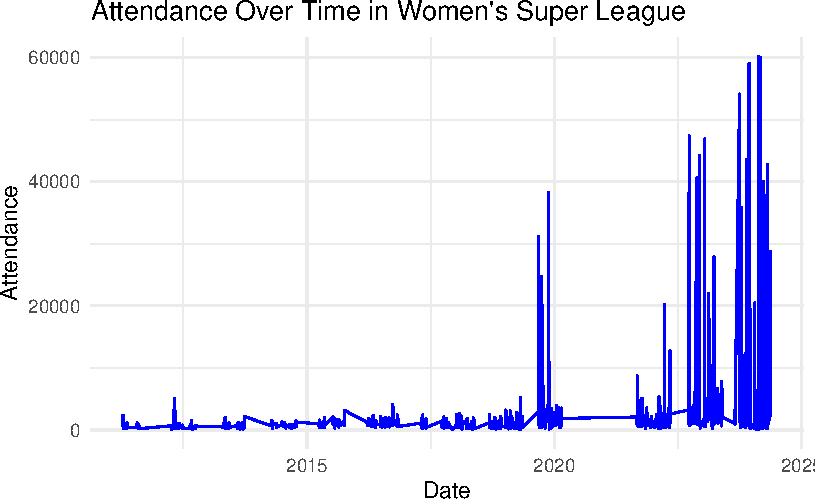
\includegraphics{paper_files/figure-pdf/fig-attendance-over-time-1.pdf}

}

\caption{\label{fig-attendance-over-time}Attendance Over Time in Women's
Super League, showing trends and notable spikes during key events.}

\end{figure}

\hypertarget{match-outcomes}{%
\subsubsection{Match Outcomes}\label{match-outcomes}}

The match outcomes variable is a categorical outcome representing
whether the home team won, the away team won, or if the match ended in a
draw. This outcome helps to assess the impact of various predictors,
such as attendance, on the likelihood of different results.

\begin{Shaded}
\begin{Highlighting}[]
\CommentTok{\# Summarizing match outcomes}
\NormalTok{match\_outcome\_summary }\OtherTok{\textless{}{-}}\NormalTok{ cleaned\_data }\SpecialCharTok{\%\textgreater{}\%}
  \FunctionTok{group\_by}\NormalTok{(result) }\SpecialCharTok{\%\textgreater{}\%}
  \FunctionTok{summarise}\NormalTok{(}
    \AttributeTok{avg\_attendance =} \FunctionTok{mean}\NormalTok{(attendance, }\AttributeTok{na.rm =} \ConstantTok{TRUE}\NormalTok{),}
    \AttributeTok{total\_matches =} \FunctionTok{n}\NormalTok{()}
\NormalTok{  )}

\CommentTok{\# Display table using tinytable for better formatting}
\CommentTok{\# tinytable::tt(match\_outcome\_summary, colnames = TRUE, rownames = FALSE)}
\end{Highlighting}
\end{Shaded}

\begin{table}

\caption{\textbf{?(caption)}}

\end{table}

\hypertarget{predictor-variables}{%
\subsection{Predictor variables}\label{predictor-variables}}

This section discusses the predictor variables used in the model. These
predictors include:

\begin{enumerate}
\def\labelenumi{\arabic{enumi}.}
\item
  Goals Scored (goals\_for): The number of goals scored by a team during
  a match. Goals are key indicators of team performance and are directly
  related to the likelihood of winning a match.
\item
  Goals Against (goals\_against): The number of goals conceded by a
  team. Fewer goals conceded generally indicates a stronger defense and
  contributes to better match outcomes.
\item
  Tier (tier): The level at which the team is playing, either in the
  Women's Super League or Championship. Teams at different tiers may
  show varied performance due to differences in competitiveness.
\end{enumerate}

\begin{Shaded}
\begin{Highlighting}[]
\CommentTok{\# Load correct dataset for predictor variables}
\NormalTok{predictor\_data }\OtherTok{\textless{}{-}} \FunctionTok{read\_parquet}\NormalTok{(here}\SpecialCharTok{::}\FunctionTok{here}\NormalTok{(}\StringTok{"data"}\NormalTok{, }\StringTok{"02{-}analysis\_data"}\NormalTok{, }\StringTok{"ewf\_appearances\_cleaned.parquet"}\NormalTok{))}

\CommentTok{\# Plotting distribution of goals scored by tier}
\NormalTok{predictor\_plot }\OtherTok{\textless{}{-}}\NormalTok{ predictor\_data }\SpecialCharTok{\%\textgreater{}\%}
  \FunctionTok{filter}\NormalTok{(}\SpecialCharTok{!}\FunctionTok{is.na}\NormalTok{(goals\_for), }\SpecialCharTok{!}\FunctionTok{is.na}\NormalTok{(tier)) }\SpecialCharTok{\%\textgreater{}\%}
  \FunctionTok{ggplot}\NormalTok{(}\FunctionTok{aes}\NormalTok{(}\AttributeTok{x =}\NormalTok{ goals\_for, }\AttributeTok{fill =} \FunctionTok{as.factor}\NormalTok{(tier))) }\SpecialCharTok{+}
  \FunctionTok{geom\_histogram}\NormalTok{(}\AttributeTok{binwidth =} \DecValTok{1}\NormalTok{, }\AttributeTok{alpha =} \FloatTok{0.7}\NormalTok{, }\AttributeTok{position =} \StringTok{"dodge"}\NormalTok{, }\AttributeTok{color =} \StringTok{"black"}\NormalTok{) }\SpecialCharTok{+}
  \FunctionTok{labs}\NormalTok{(}\AttributeTok{title =} \StringTok{"Distribution of Goals Scored by Tier"}\NormalTok{, }\AttributeTok{x =} \StringTok{"Goals Scored"}\NormalTok{, }\AttributeTok{y =} \StringTok{"Frequency"}\NormalTok{) }\SpecialCharTok{+}
  \FunctionTok{theme\_minimal}\NormalTok{()}

\NormalTok{predictor\_plot}
\end{Highlighting}
\end{Shaded}

\begin{figure}[H]

{\centering 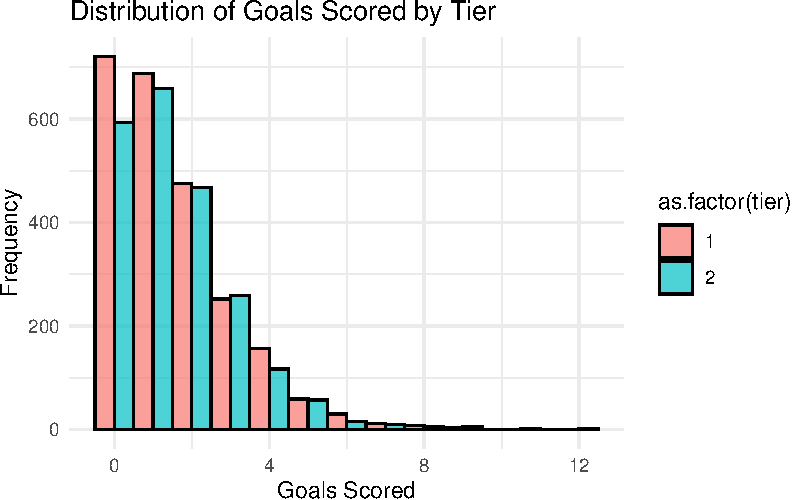
\includegraphics{paper_files/figure-pdf/fig-predictor-distribution-1.pdf}

}

\caption{\label{fig-predictor-distribution}Distribution of Goals Scored
and Goals Against by Team Tier}

\end{figure}

\hypertarget{sec-model}{%
\section{Model}\label{sec-model}}

The goal of our modeling strategy is twofold. Firstly, we seek to
understand how match characteristics affect team performance. Secondly,
we aim to predict team success based on key performance indicators such
as goals scored, goals conceded, and attendance.

Here we briefly describe the Bayesian analysis model used to investigate
these questions. Background details and diagnostics are included in
Appendix~\ref{sec-model-details}.

\hypertarget{model-set-up}{%
\subsection{Model set-up}\label{model-set-up}}

Define \(y_i\) as the number of points that a team earns in a given
season. Then \(eta_i\) represents goals scored and \(\gamma_i\)
represents goals conceded, both measured per match.

\begin{align}
y_i|\mu_i, \sigma &\sim \text{Normal}(\mu_i, \sigma) \
\mu_i &= \alpha + \beta_i \cdot \text{goals_for} + \gamma_i \cdot \text{goals_against} + \text{tier} \
\alpha &\sim \text{Normal}(0, 2.5) \
\beta &\sim \text{Normal}(0, 2.5) \
\gamma &\sim \text{Normal}(0, 2.5) \
\sigma &\sim \text{Exponential}(1)
\end{align}lpha + \beta\_i \cdot \text{goals_for} + \gamma\_i
\cdot \text{goals_against} + \text{tier}\\
\alpha \&\sim \text{Normal}(0, 2.5)\\
\beta \&\sim \text{Normal}(0, 2.5)\\
\gamma \&\sim \text{Normal}(0, 2.5)\\
\sigma \&\sim \text{Exponential}(1) \textbackslash end\{align\}

We run the model in R (R Core Team 2023) using the rstanarm package of
Goodrich et al. (2022). We use the default priors from
\texttt{rstanarm}.

\hypertarget{model-justification}{%
\subsubsection{Model justification}\label{model-justification}}

We expect a positive relationship between the number of goals scored and
the points a team earns. Conversely, we expect a negative relationship
between goals conceded and points earned. These relationships capture
the offensive and defensive capabilities of a team.

\hypertarget{sec-results}{%
\section{Results}\label{sec-results}}

Our results are summarized in \textbf{?@tbl-modelresults}. The model
provides an understanding of the relationships between goals scored,
goals conceded, and overall team performance.

\begin{verbatim}
Loading required package: Rcpp
\end{verbatim}

\begin{verbatim}
This is rstanarm version 2.32.1
\end{verbatim}

\begin{verbatim}
- See https://mc-stan.org/rstanarm/articles/priors for changes to default priors!
\end{verbatim}

\begin{verbatim}
- Default priors may change, so it's safest to specify priors, even if equivalent to the defaults.
\end{verbatim}

\begin{verbatim}
- For execution on a local, multicore CPU with excess RAM we recommend calling
\end{verbatim}

\begin{verbatim}
  options(mc.cores = parallel::detectCores())
\end{verbatim}

\begin{table}

\caption{\textbf{?(caption)}}

\end{table}

\hypertarget{discussion}{%
\section{Discussion}\label{discussion}}

\hypertarget{sec-first-point}{%
\subsection{Understanding the Factors that Drive Match
Attendance}\label{sec-first-point}}

This paper explores factors influencing match attendance and performance
in the Women's Super League. One of the key findings is that attendance
has generally increased over time, with major events and international
tournaments serving as pivotal moments that boost interest in women's
football. Understanding what drives this interest allows league
organizers to align promotional efforts with these catalysts.

The correlation between attendance and home team success suggests that
fan presence can impact match outcomes, likely by providing a
motivational boost to players. The findings here indicate that
increasing audience engagement could have tangible benefits for home
team performance.

\hypertarget{the-relationship-between-goals-and-team-success}{%
\subsection{The Relationship Between Goals and Team
Success}\label{the-relationship-between-goals-and-team-success}}

Another key observation is the direct impact of goals scored and goals
conceded on team standings. Goals scored positively affect match
outcomes, as expected, while goals conceded correlate negatively with
team success. These results confirm the intuitive idea that both
offensive and defensive abilities are crucial for a team's performance.
It is not enough to simply score goals---preventing the opponent from
scoring also plays an important role.

Moreover, the analysis of attendance reveals that larger crowds tend to
coincide with better performances for the home team. This finding
highlights the potential advantage that crowd support can provide,
supporting the concept of ``home-field advantage'' in sports.

\hypertarget{implications-for-teams-and-organizers}{%
\subsection{Implications for Teams and
Organizers}\label{implications-for-teams-and-organizers}}

The results suggest that teams should focus on improving both offensive
capabilities and defensive solidity to succeed. Beyond game tactics,
teams and league organizers should continue to work on increasing fan
attendance, as the presence of spectators has a clear impact on home
team success. This can be achieved through better marketing, improved
game day experiences, and leveraging international events to draw in
larger audiences.

For organizers, these insights are valuable for shaping promotional
strategies that increase attendance, leveraging key calendar events, and
enhancing audience experience, thereby boosting overall league
engagement and team performance.

\hypertarget{sec-weaknesses}{%
\subsection{Weaknesses and Next Steps}\label{sec-weaknesses}}

There are several limitations in the current study that should be
addressed in future research. Firstly, the dataset used only spans a
certain period, which may limit the generalizability of these results.
Extending the analysis to include more seasons would provide a better
understanding of longer-term trends.

Another limitation is the absence of player-specific performance
metrics. Incorporating individual-level data, such as player fatigue or
injuries, would add depth to our understanding of what drives match
outcomes. Future models could incorporate additional predictors to
improve predictive power and capture the complex dynamics of match
performance.

Further research should also consider qualitative factors like weather
conditions or managerial changes, which could have significant effects
on match outcomes but are not captured in the current quantitative
analysis. It would also be useful to explore the impact of specific
international events on audience engagement to better understand how
these events can be utilized for marketing and promotion.

\newpage

\appendix

\hypertarget{appendix}{%
\section*{Appendix}\label{appendix}}
\addcontentsline{toc}{section}{Appendix}

\hypertarget{additional-data-details}{%
\subsection{Additional Data Details}\label{additional-data-details}}

The English Women's Football (EWF) Database provided detailed match,
attendance, and standings data. This database includes metrics such as
match outcomes, goals for and against, attendance, and standings, which
were all used in the analysis. Data cleaning and filtering steps were
performed to ensure consistency and reliability in the findings
presented.

\hypertarget{sec-model-details}{%
\subsection{Model Details}\label{sec-model-details}}

\hypertarget{posterior-predictive-check}{%
\subsubsection{Posterior Predictive
Check}\label{posterior-predictive-check}}

In Figure~\ref{fig-ppcheckandposteriorvsprior}, we implement a posterior
predictive check to evaluate how well the model fits the data. This
helps to determine if the model is appropriately capturing the patterns
in the observed data.

In Figure~\ref{fig-ppcheckandposteriorvsprior}, we compare the posterior
distributions with the prior distributions. The comparison shows how the
data has influenced the model's parameters, providing insight into the
extent to which our priors were updated by the observed data.

\begin{figure}

\begin{minipage}[t]{0.50\linewidth}

{\centering 

\raisebox{-\height}{

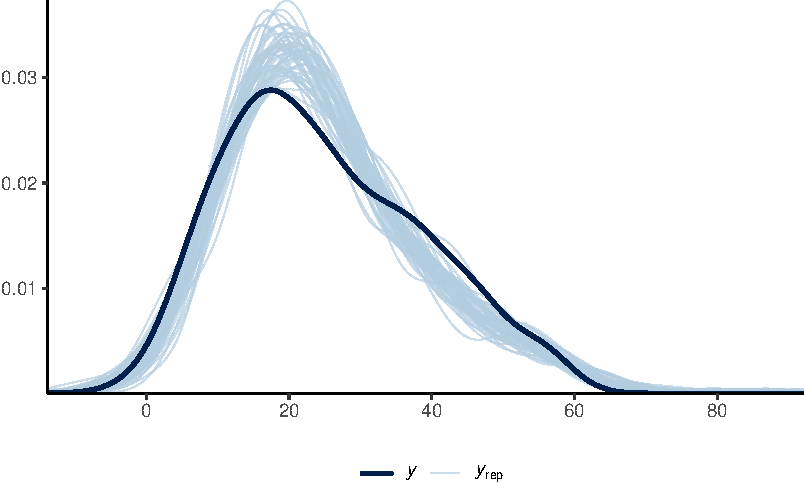
\includegraphics{paper_files/figure-pdf/fig-ppcheckandposteriorvsprior-1.pdf}

}

}

\subcaption{\label{fig-ppcheckandposteriorvsprior-1}Posterior prediction
check}
\end{minipage}%
%
\begin{minipage}[t]{0.50\linewidth}

{\centering 

\raisebox{-\height}{

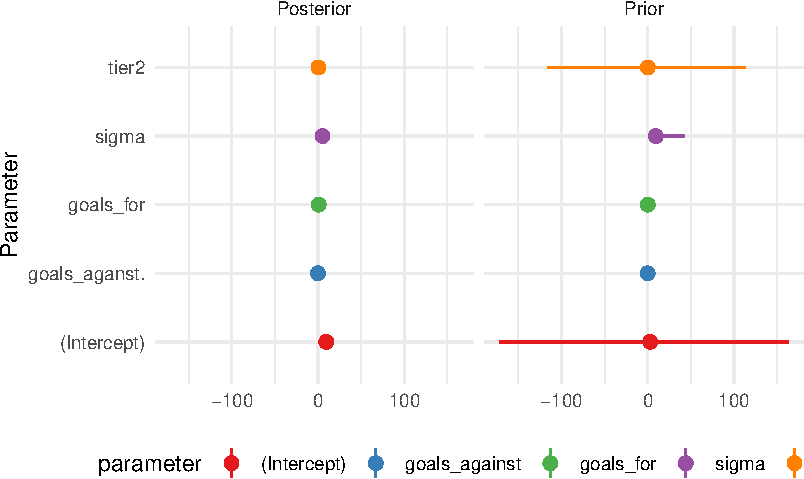
\includegraphics{paper_files/figure-pdf/fig-ppcheckandposteriorvsprior-2.pdf}

}

}

\subcaption{\label{fig-ppcheckandposteriorvsprior-2}Comparing the
posterior with the prior}
\end{minipage}%

\caption{\label{fig-ppcheckandposteriorvsprior}Examining how the model
fits and how it is affected by the data}

\end{figure}

\hypertarget{diagnostics}{%
\subsection{Diagnostics}\label{diagnostics}}

Figure~\ref{fig-stanareyouokay} shows the trace plot of the MCMC samples
for key parameters. The traces suggest that the chains have mixed well
and reached stationarity, indicating good convergence properties.

Figure~\ref{fig-stanareyouokay} also provides the Rhat diagnostic plot.
Rhat values close to 1 indicate that the model has converged
appropriately.

\begin{figure}

\begin{minipage}[t]{0.50\linewidth}

{\centering 

\raisebox{-\height}{

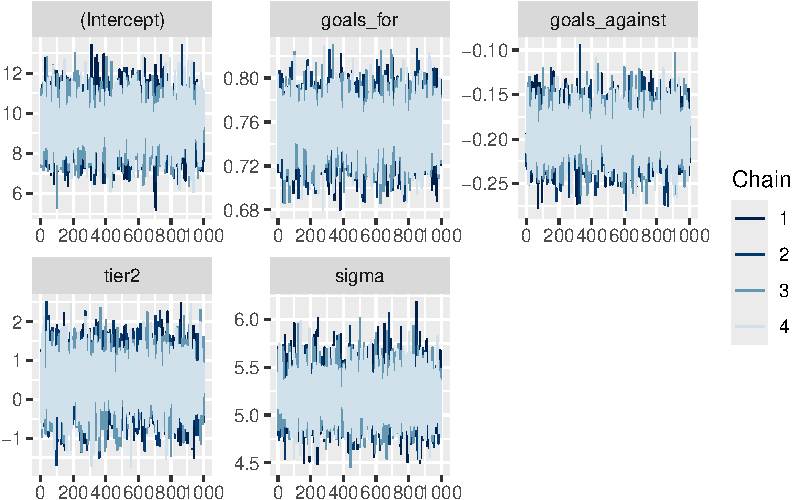
\includegraphics{paper_files/figure-pdf/fig-stanareyouokay-1.pdf}

}

}

\subcaption{\label{fig-stanareyouokay-1}Trace plot}
\end{minipage}%
%
\begin{minipage}[t]{0.50\linewidth}

{\centering 

\raisebox{-\height}{

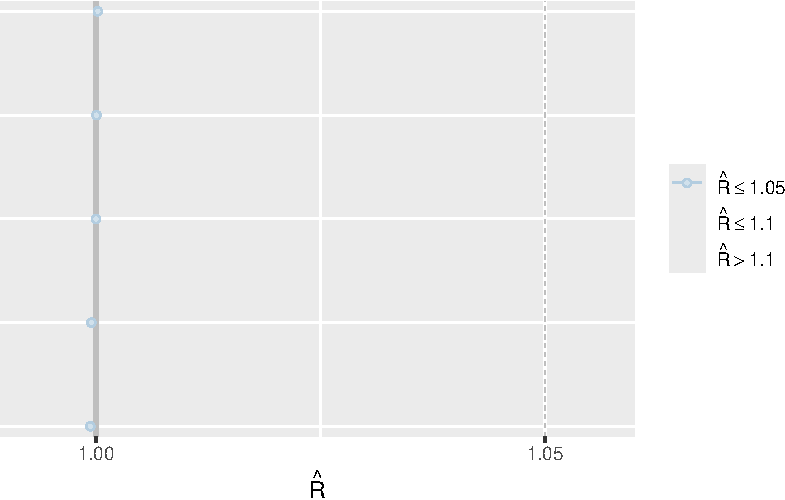
\includegraphics{paper_files/figure-pdf/fig-stanareyouokay-2.pdf}

}

}

\subcaption{\label{fig-stanareyouokay-2}Rhat plot}
\end{minipage}%

\caption{\label{fig-stanareyouokay}Checking the convergence of the MCMC
algorithm}

\end{figure}

\newpage

\hypertarget{references}{%
\section*{References}\label{references}}
\addcontentsline{toc}{section}{References}

\hypertarget{refs}{}
\begin{CSLReferences}{1}{0}
\leavevmode\vadjust pre{\hypertarget{ref-tellingstories}{}}%
Alexander, Rohan. 2023. \emph{Telling Stories with Data}. Chapman;
Hall/CRC. \url{https://tellingstorieswithdata.com/}.

\leavevmode\vadjust pre{\hypertarget{ref-rstanarm}{}}%
Goodrich, Ben, Jonah Gabry, Imad Ali, and Sam Brilleman. 2022.
{``{rstanarm: {Bayesian} applied regression modeling via {Stan}}.''}
\url{https://mc-stan.org/rstanarm/}.

\leavevmode\vadjust pre{\hypertarget{ref-citeR}{}}%
R Core Team. 2023. \emph{{R: A Language and Environment for Statistical
Computing}}. Vienna, Austria: R Foundation for Statistical Computing.
\url{https://www.R-project.org/}.

\end{CSLReferences}



\end{document}
